\let\negmedspace\undefined
\let\negthickspace\undefined
\documentclass[journal]{IEEEtran}
\usepackage[a5paper, margin=10mm, onecolumn]{geometry}
\usepackage{lmodern} % Ensure lmodern is loaded for pdflatex
\usepackage{tfrupee} % Include tfrupee package

\setlength{\headheight}{1cm} % Set the height of the header box
\setlength{\headsep}{0mm}  % Set the distance between the header box and the top of the text

\usepackage{csquotes}
\usepackage{gvv-book}
\usepackage{gvv}
\usepackage{circuitikz}
\usepackage{cite}
\usepackage{amsmath,amssymb,amsfonts,amsthm}
\usepackage{algorithmic}
\usepackage{graphicx}
\usepackage{textcomp}
\usepackage{xcolor}
\usepackage{txfonts}
\usepackage{listings}
\usepackage{enumitem}
\usepackage{mathtools}
\usepackage{gensymb}
\usepackage{comment}
\usepackage[breaklinks=true]{hyperref}
\usepackage{tkz-euclide} 
\usepackage{listings}
% \usepackage{gvv}                                        
\def\inputGnumericTable{}                                 
\usepackage[latin1]{inputenc}                                
\usepackage{color}                                            
\usepackage{array}                                            
\usepackage{longtable}                                       
\usepackage{calc}                                             
\usepackage{multirow}                                         
\usepackage{hhline}                                           
\usepackage{ifthen}                                           
\usepackage{lscape}
\usepackage{caption}
\usepackage{tikz}
\usetikzlibrary{patterns}


\begin{document}

\begin{center}
    \textbf{GATE 2012 Online Examination} \\[0.3em]
    \textbf{AG : AGRICULTURAL ENGINEERING} \\[1em]
    \begin{tabular}{l@{\qquad}r}
        \textit{Duration:} Three Hours & \textit{Maximum Marks:} 100
    \end{tabular}
\end{center}


\section*{Q.1 -- Q.25 carry one mark each.}

\begin{enumerate}
\item
The matrix 
\myvec{
0 & 2 & -3 \\
-2 & 0 & 4 \\
3 & -4 & 0 \\
}
is 
\begin{enumerate}
\begin{multicols}{2}
\item diagonal
\item symmetric
\item skew symmetric
\item triangular
\end{multicols}
\end{enumerate}
\hfill(GATE AG 2012)\\

\medskip

\item
The line $y = x-1$ can be expressed in polar coordinates $(r, \theta)$ as
\begin{enumerate}
\begin{multicols}{2}
\item $r = \cos \theta$
\item $r = \sin \theta$
\item $r (\cos \theta + \sin \theta) = 1$
\item $r (\cos \theta - \sin \theta) = 1$
\end{multicols}
\end{enumerate}
\hfill(GATE AG 2012)\\

\medskip

\item
The type of pump used in forced water cooling system of a tractor engine is
\begin{enumerate}
\begin{multicols}{2}
\item piston
\item centrifugal
\item gear
\item vane
\end{multicols}
\end{enumerate}
\hfill(GATE AG 2012)\\

\medskip

\item
Which one of the following statements is NOT appropriate regarding cone index
\begin{enumerate}
\begin{multicols}{2}
\item It reflects strength of soil
\item It is a composite parameter
\item It is dimensionless
\item It is measured at a constant penetration rate of 30 mm/s
\end{multicols}
\end{enumerate}
\hfill(GATE AG 2012)\\

\medskip

\item
The draft and total power requirement of a rotary cultivator operating in concurrent mode as compared to a spring tyne cultivator of equal cutting width under the same operating conditions, respectively are
\begin{enumerate}
\begin{multicols}{2}
\item higher and higher
\item lower and lower
\item lower and higher
\item higher and lower
\end{multicols}
\end{enumerate}
\hfill(GATE AG 2012)\\

\medskip

\item
The soil erodibility factor needs to be determined for use in the universal soil loss equation. The length, in m, and slope, in \% of the experimental plot to be used for this purpose, respectively are
\begin{enumerate}
\begin{multicols}{2}
\item 19, 12
\item 21, 11
\item 22, 9
\item 23, 8
\end{multicols}
\end{enumerate}
\hfill(GATE AG 2012)\\

\medskip

\item
The difference between Fore Bearing and Back Bearing of a traverse line is
\begin{enumerate}
\begin{multicols}{2}
\item exactly $90^\circ$
\item less than $180^\circ$
\item exactly $180^\circ$
\item greater than $180^\circ$
\end{multicols}
\end{enumerate}
\hfill(GATE AG 2012)\\

\medskip

\item
A pumping device that combines the advantages of both centrifugal and reciprocating pumps is known as
\begin{enumerate}
\begin{multicols}{2}
\item air lift pump
\item hydraulic ram
\item jet pump
\item rotary pump
\end{multicols}
\end{enumerate}
\hfill(GATE AG 2012)\\

\medskip

\item
If $\nu$ is the kinematic viscosity of air -- water vapour mixture and $D_{AB}$ is the mass diffusivity of water vapour in air then the ratio $\nu/D_{AB}$ is known as
\begin{enumerate}
\begin{multicols}{2}
\item Stanton number
\item Prandtl number
\item Schmidt number
\item Sherwood number
\end{multicols}
\end{enumerate}
\hfill(GATE AG 2012)\\

\medskip

\item
Work index in size reduction can be obtained by multiplying Bond's energy constant with
\begin{enumerate}
\begin{multicols}{2}
\item 10
\item $\sqrt{10}$
\item $\sqrt[3]{10}$
\item $\sqrt{10}$
\end{multicols}
\end{enumerate}
\hfill(GATE AG 2012)\\

\medskip

\item
The tangent line to $y = f(x)$ at the point $(x_0, y_0)$, assuming $f'(x) \neq 0$, intersects the $x$ axis at
\begin{enumerate}
\begin{multicols}{2}
\item $(x_0 - [y_0/f'(x_0)], 0)$
\item $(x_0 + [y_0/f'(x_0)], 0)$
\item $(x_0 - [f'(x_0)/y_0], 0)$
\item $(x_0 + [f'(x_0)/y_0], 0)$
\end{multicols}
\end{enumerate}
\hfill(GATE AG 2012)\\

\medskip

\item
Approximate percentage of scores that fall within $\pm \sigma$ (standard deviation) of the mean in a normal distribution is 
\begin{enumerate}
\begin{multicols}{2}
\item 34
\item 68
\item 95
\item 99
\end{multicols}
\end{enumerate}
\hfill(GATE AG 2012)\\

\medskip

\item
The integrating factor of the differential equation $(x+1)\, \dfrac{dy}{dx} - y = \sin x$ is
\begin{enumerate}
\begin{multicols}{2}
\item $x$
\item $(x+1)$
\item $1/x$
\item $1/(x+1)$
\end{multicols}
\end{enumerate}
\hfill(GATE AG 2012)\\

\medskip

\item
The constituent of producer gas which occupies the highest percentage by volume and helps in increasing its overall calorific value is
\begin{enumerate}
\begin{multicols}{2}
\item CO
\item CO$_2$
\item H$_2$
\item CH$_4$
\end{multicols}
\end{enumerate}
\hfill(GATE AG 2012)\\

\medskip

\item
During field operation, the shank of a tractor drawn rigid tyne sweep type cultivator is mainly subjected to
\begin{enumerate}
\begin{multicols}{2}
\item bending
\item shear
\item torsion
\item bending and torsion
\end{multicols}
\end{enumerate}
\hfill(GATE AG 2012)\\

\medskip

\item
A slider is moving on a straight link at a sliding velocity of $0.5$ m s$^{-1}$. The straight link is pivoted at one end and makes angular movement at a rate of $1.0$ rad s$^{-1}$. Coriolis acceleration of the slider in m s$^{-2}$ is
\begin{enumerate}
\begin{multicols}{2}
\item 0.25
\item 0.50
\item 1.00
\item 4.00
\end{multicols}
\end{enumerate}
\hfill(GATE AG 2012)\\

\medskip

\item
The power developed and the exhaust gas temperature of a diesel engine compared to a spark ignition engine of the same size and running at the same speed respectively, are
\begin{enumerate}
\begin{multicols}{2}
\item higher and lower
\item higher and higher
\item lower and higher
\item lower and lower
\end{multicols}
\end{enumerate}
\hfill(GATE AG 2012)\\

\medskip

\item
In a semi-modular outlet, the discharge
\begin{enumerate}
\begin{multicols}{2}
\item is independent of water levels in the distributary and the water course
\item depends upon the water levels of both distributary and water course
\item depends upon the water level in the distributary
\item depends upon the water level in the water course
\end{multicols}
\end{enumerate}
\hfill(GATE AG 2012)\\

\medskip

\item
The relationship between outflow $Q$ in m$^3$ s$^{-1}$ and storage $S$ in m$^3$ for an emergency spillway in a reservoir is $Q=S/4000$. Inflow, outflow and storage are assumed to be zero at time $t=0$. If the inflow rate is $300$ m$^{3}$ s$^{-1}$ at the end of $t=3$ hours, the outflow rate in m$^3$ s$^{-1}$ is
\begin{enumerate}
\begin{multicols}{2}
\item 152.84
\item 164.84
\item 172.34
\item 184.84
\end{multicols}
\end{enumerate}
\hfill(GATE AG 2012)\\

\medskip

\item
A trapezoidal grassed waterway is constructed along a longitudinal gradient of 4\%. If the cross - sectional area of flow is 1.52 m$^2$, wetted perimeter is 12.5 m and Manning's $n$ for the waterway is $0.04$ m$^{-1/3}$ s, the flow through the waterway in m$^3$ s$^{-1}$ is
\begin{enumerate}
\begin{multicols}{2}
\item 1.9
\item 2.1
\item 2.3
\item 2.5
\end{multicols}
\end{enumerate}
\hfill(GATE AG 2012)\\

\medskip

\item
 A single acting reciprocating pump discharges 3.5 litres of water per second at 40 rpm. The pump has a piston diameter of 150 mm and a stroke of 300 mm. The percentage slip is
\begin{enumerate}
\begin{multicols}{2}
\item 0.85
\item 1.97
\item 3.53
\item 6.05
\end{multicols}
\end{enumerate}
\hfill(GATE AG 2012)\\

\medskip

\item
 A pair of parallel glass panes, each of 3 mm thickness traps 2 mm layer of stagnant air. Thermal conductivities of glass and air are 0.5 and 0.02 W m$^{-1}$ K$^{-1}$, respectively. If the film heat transfer coefficient of air is 10 W m$^{-2}$ K$^{-1}$, then Biot Number is
\begin{enumerate}
\begin{multicols}{2}
\item 1.50
\item 1.00
\item 0.06
\item 0.04
\end{multicols}
\end{enumerate}
\hfill(GATE AG 2012)\\

\medskip

\item
 Two small parallel plane surface cassettes, each measuring 4 mm $\times$ 4 mm are placed 0.5 m apart (centre to centre) with 30$^{\circ}$ angle between the radial distance and both the surface normals. The view factor between the two surfaces is
\begin{enumerate}
\begin{multicols}{2}
\item $1.53 \times 10^{-5}$
\item $1.76 \times 10^{-5}$
\item $3.82 \times 10^{-3}$
\item $4.41 \times 10^{-3}$
\end{multicols}
\end{enumerate}
\hfill(GATE AG 2012)\\

\medskip

\item
 Tomato catsup with 10 Pa.s$^n$ consistency coefficient and 0.8 flow behaviour index is flowing in a pipe. Generalized coefficient of viscosity of catsup, in Pa.s$^n$ is
\begin{enumerate}
\begin{multicols}{2}
\item 2.66
\item 6.93
\item 15.91
\item 23.87
\end{multicols}
\end{enumerate}
\hfill(GATE AG 2012)\\

\medskip

\item
 A packed bed of 480 kg solid particles having particle size of 0.15 mm and density of 800 kg/m$^3$ is fluidized using air at 25$^\circ$C and 1 atmospheric pressure. If the cross section of the empty bed is 0.45 m$^2$ and voidage at minimum fluidizing condition is 0.5, the minimum height of the fluidized bed, in m is
\begin{enumerate}
\begin{multicols}{2}
\item 7.4
\item 5.4
\item 2.7
\item 1.0
\end{multicols}
\end{enumerate}
\hfill(GATE AG 2012)\\

\medskip

\vspace{1em}
\noindent
\textbf{Q. 26 to Q. 55 carry two marks each.}

\item
 The value of
\begin{align}
\int_0^{\pi/2} \cos x \, dx
\end{align}
using trapezoidal rule with two equal intervals is
\begin{enumerate}
\begin{multicols}{2}
\item 0.95
\item 1.00
\item 1.22
\item 1.29
\end{multicols}
\end{enumerate}
\hfill(GATE AG 2012)\\

\medskip

\item
 A tractor power take-off (PTO) driven stationary peg tooth type wheat thresher operating at a cylinder speed of 540 rpm requires a torque of 250 Nm at PTO. The minimum net engine power required, in kW is
\begin{enumerate}
\begin{multicols}{2}
\item 13
\item 16
\item 18
\item 21
\end{multicols}
\end{enumerate}
\hfill(GATE AG 2012)\\

\medskip

\item
 A border strip of $8 \times 250$ m is being irrigated by a border stream of 50 lps. The infiltration capacity of the soil is 25 mm h$^{-1}$ (assumed to be constant throughout the period of irrigation). The average depth of the advancing sheet of water over the land is 70 mm. The time required to irrigate the border strip, in minutes, will be
\begin{enumerate}
\begin{multicols}{2}
\item 16.7
\item 25.7
\item 54.7
\item 67.7
\end{multicols}
\end{enumerate}
\hfill(GATE AG 2012)\\

\medskip

\item
 Decimal reduction times for \textit{Bacillus subtilis} are 37 s and 12 s at temperatures of $120^\circ$C and $125^\circ$C, respectively. The temperature rise, in $^\circ$C, necessary to reduce the first value of decimal reduction time at $120^\circ$C by a factor of 10 is
\begin{enumerate}
\begin{multicols}{2}
\item 7.18
\item 10.36
\item 13.06
\item 16.07
\end{multicols}
\end{enumerate}
\hfill(GATE AG 2012)\\

\medskip

\item
 A tall silo having height to diameter ratio of 2 is holding 480 tons wheat of bulk density $960$ kg m$^{-3}$. The angle of internal friction for wheat is $25^\circ$ and for wheat and wall surface is $24^\circ$. Applying Airy formula, the maximum lateral pressure in kPa at the bottom of the bin section is
\begin{enumerate}
\begin{multicols}{2}
\item 40.24
\item 41.79
\item 42.83
\item 42.92
\end{multicols}
\end{enumerate}
\hfill(GATE AG 2012)\\

\medskip


\noindent
\item
The eigenvalues of the matrix
\myvec{
6 & 1 \\
-2 & 3}
are
\begin{enumerate}
\begin{multicols}{2}
\item (3, 6) 
\item (1, -2)
\item (5, 4) 
\item (1, 6)
\end{multicols}
\end{enumerate}
\hfill(GATE AG 2012)\\

\medskip


\item
 If $f'(x) = e^x$ and $f(0)=5$, then from Mean Value Theorem, the value of $f(1)$ lies between
\begin{enumerate}
\begin{multicols}{2}
\item 2 and $2+e$
\item 3 and $(2+e)$
\item 3 and $(3+e)$
\item 6 and $(5+e)$
\end{multicols}
\end{enumerate}
\hfill(GATE AG 2012)\\

\medskip

\item
 The inverse Laplace Transform of $\dfrac{s^2}{(s-3)^3}$ can be written as $\dfrac{e^{3t}}{2}[A t^2+Bt+C]$. The values of $A$, $B$ and $C$, respectively are
\begin{enumerate}
\begin{multicols}{2}
\item 3, 5 and 7
\item 2, 10 and 12
\item 10, 12 and 4
\item 9, 12 and 2
\end{multicols}
\end{enumerate}
\hfill(GATE AG 2012)\\

\medskip

\item
 A two wheel drive tractor, weighing 15.84 kN with a wheel base of 2160 mm, has the static weight divided between the front and rear axles in the ratio of 30 : 70 on a horizontal level surface. The hitch point is at a height of 700 mm from the ground and at a horizontal distance of 120 mm to the rear side from the center of the rear axle. Pull acts at an angle of $12^\circ$ downwards from the horizontal. The maximum pull in kN, when the front wheels would just start rising from the ground is
\begin{enumerate}
\begin{multicols}{2}
\item 1.48
\item 14.46
\item 39.04
\item 85.54
\end{multicols}
\end{enumerate}
\hfill(GATE AG 2012)\\

\medskip

\item
 A horizontal axis drag type wind mill with square blades and a horizontal axis lift type wind mill with airfoil section blades having same rotor size are installed at a height of 10 m above the ground. The average wind speed is 25 km h$^{-1}$. The maximum power coefficient for drag type and lift type wind mills is 0.148 and 0.593, respectively. If the maximum power extracted by drag type wind mill is 5 kW, the corresponding power extracted by lift type wind mill, in kW is
\begin{enumerate}
\begin{multicols}{2}
\item 8.43
\item 12.63
\item 18.03
\item 20.03
\end{multicols}
\end{enumerate}
\hfill(GATE AG 2012)\\

\medskip

\item
 The thresher of a wheat combine harvester has an optimal throughput capacity of 2400 kg (crop) per hour. The harvester has a forward velocity of 4.5 km h$^{-1}$. Sample tests have revealed that the yield of crop in the field is 3000 kg (grain) per ha. Grain to straw ratio is 60:40. If the above throughput is to be maintained, the width of cut of the harvester in m, neglecting turning losses, is
\begin{enumerate}
\begin{multicols}{2}
\item 0.71
\item 1.07
\item 1.78
\item 2.96
\end{multicols}
\end{enumerate}
\hfill(GATE AG 2012)\\

\medskip

\item
 In a disc clutch, the inside and outside radii of the clutch plate are 50 and 100 mm, respectively. If the axial force exerted on the disc is 4 kN, the maximum pressure experienced by the clutch plate in N mm$^{-2}$ under uniform wear conditions is
\begin{enumerate}
\begin{multicols}{2}
\item 0.13
\item 0.17
\item 0.25
\item 0.51
\end{multicols}
\end{enumerate}
\hfill(GATE AG 2012)\\

\medskip

\item
 A regime channel carrying a discharge of 25 m$^3$ s$^{-1}$ is designed using Lacey's regime theory. The side slope of the channel is 1/2 H:1 V, and Lacey’s silt factor is unity. The bottom width and depth of flow in the channel, in m, respectively are
\begin{enumerate}
\begin{multicols}{2}
\item 20.26, 1.38
\item 20.26, 1.56
\item 23.75, 1.56
\item 32.78, 1.56
\end{multicols}
\end{enumerate}
\hfill(GATE AG 2012)\\

\medskip

\item
 Flow is taking place through a layered soil system, having two homogeneous soils M and N, as shown in the figure. The head lost in soil N is 20 times the head lost in soil M.

\begin{figure}[h]
    \centering
    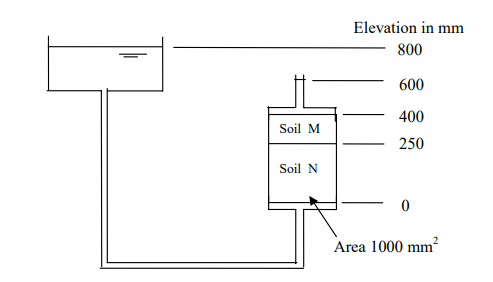
\includegraphics[width=0.7\columnwidth]{Figs/Screenshot 2025-08-18 093210.png}
    \caption{}
    \label{fig 1}
\end{figure}

\medskip

If the permeability of soil M is $3\times 10^{-4}$ mm s$^{-1}$, the permeability of soil N, in mm s$^{-1}$, will be
\begin{enumerate}
\begin{multicols}{2}
\item $4\times 10^{-4}$
\item $3\times 10^{-4}$
\item $2.5\times 10^{-5}$
\item $1.5\times 10^{-5}$
\end{multicols}
\end{enumerate}
\hfill(GATE AG 2012)\\

\medskip

\item
 A trapezoidal canal, having a bottom width of 5.0 m and a side slope of 1 H : 1 V, is carrying a discharge of 20 m$^3$ s$^{-1}$. The critical depth, in m, is
\begin{enumerate}
\begin{multicols}{2}
\item 1.09
\item 1.18
\item 2.12
\item 2.62
\end{multicols}
\end{enumerate}
\hfill(GATE AG 2012)\\

\medskip

\item
 A 200 mm well fully penetrates a confined aquifer. After a long period of pumping at a rate of 1400 litres per minute, the drawdowns in the observation wells located at 25 m and 40 m from the pumping well are found to be 2.6 m and 1.9 m, respectively. The transmissivity of the aquifer in m$^2$ day$^{-1}$ is
\begin{enumerate}
\begin{multicols}{2}
\item 190
\item 198
\item 206
\item 215
\end{multicols}
\end{enumerate}
\hfill(GATE AG 2012)\\

\medskip

\item
 Tile drains have to be installed in an agricultural land having soil permeability of $2.3\times 10^{-3}$ mm s$^{-1}$. An impermeable stratum exists at 3.2 m below the land surface, and it is desired to keep the water level at least 1.0 m below the land surface. The average discharge of the drainage system is 2.0 mm day$^{-1}$. If the tile drains are planned to be placed at 1.5 m below the land surface, the drain spacing in m, assuming the equivalent depth to be the same as the tile depth, is
\begin{enumerate}
\begin{multicols}{2}
\item 10.6
\item 12.4
\item 13.9
]\item 19.7
\end{multicols}
\end{enumerate}
\hfill(GATE AG 2012)\\

\medskip

\item
 It is proposed to construct bench terraces on a 10\% hill slope. If the batter slope is $1/2$ H : 1 V, the percentage area that will be lost for cultivation due to bench terracing is
\begin{enumerate}
\begin{multicols}{2}
\item 4.68
\item 5.47
\item 6.25
\item 6.78
\end{multicols}
\end{enumerate}
\hfill(GATE AG 2012)\\

\medskip

\item
 Air at 70~$^\circ$C and 0.015 humidity ratio is cooled adiabatically by spraying water. The final temperature of the air is 55~$^\circ$C. Specific heat capacities of dry air and water vapour are 1.005 and 1.88 kJ kg$^{-1}$ K$^{-1}$, respectively and latent heat of vapourization of water at 0~$^\circ$C is 2501.7 kJ kg$^{-1}$. The absolute humidity of the outlet air, in kg water vapour per kg dry air is
\begin{enumerate}
\begin{multicols}{2}
\item 0.017
\item 0.019
\item 0.021
\item 0.023
\end{multicols}
\end{enumerate}
\hfill(GATE AG 2012)\\

\medskip

\item
 Final mass flow rate of osmotically dehydrated cherries after finish drying from 18\% dry basis moisture content to 11.5\% wet basis moisture content is 5000 kg per hour. The dryer efficiency is 70\%, latent heat of vaporization is 2345 kJ kg$^{-1}$, specific heat of air is 1.005 kJ kg$^{-1}$ K$^{-1}$, drying temperature is 50~$^\circ$C and the specific volume of ambient air at 25~$^\circ$C is 0.866 m$^3$ kg$^{-1}$. The necessary air flow requirement for the drying system in m$^3$ min$^{-1}$ is
\begin{enumerate}
\begin{multicols}{2}
\item 477
\item 587
\item 625
\item 702
\end{multicols}
\end{enumerate}
\hfill(GATE AG 2012)\\

\medskip

\item
 A single effect vacuum evaporator has 100 tubes of 25 mm diameter. One thousand kg feed of milk per hour with 15\% TS is concentrated to 20\% TS in the evaporator. Film heat transfer coefficients on either sides of the tube are 5000 and 800 W m$^{-2}$ K$^{-1}$. Thermal conductivity of 1.5 mm thick SS tubes is 15 W m$^{-1}$ K$^{-1}$. Latent heat of vaporization under vacuum is 2309 kJ kg$^{-1}$. For 10~$^\circ$C temperature difference across the tube wall, the height of each tube, in m is
\begin{enumerate}
\begin{multicols}{2}
\item 1.36
\item 2.13
\item 2.56
\item 3.17
\end{multicols}
\end{enumerate}
\hfill(GATE AG 2012)\\

\medskip

\item
 One thousand units of mixed fruit bar, each weighing 100 g with a surface area of 0.01 m$^2$, are frozen from 70~$^\circ$C molten mass condition to $-$20~$^\circ$C frozen storage condition within 3 hours. The specific heat capacity values of the bar are 3.6 kJ kg$^{-1}$ K$^{-1}$ and 1.97 kJ kg$^{-1}$ K$^{-1}$ before and after freezing point (0~$^\circ$C) respectively. If the latent heat of crystallization is 250 kJ kg$^{-1}$, the cooling capacity of the refrigeration unit required in tons of refrigeration is
\begin{enumerate}
\begin{multicols}{2}
\item 0.77
\item 1.43
\item 1.66
\item 4.32
\end{multicols}
\end{enumerate}
\hfill(GATE AG 2012)\\

\medskip

\section*{Common Data Questions}

\textbf{Common Data for Questions 48 and 49:}

A diesel engine running in dual fuel mode with diesel as pilot fuel and producer gas as primary fuel produces 3.5 kW at rated engine speed and is coupled directly to a generator for producing electricity. The amount of diesel and producer gas consumed per hour is 460 ml and 12.5 m$^3$, respectively.

\item
 Assuming calorific value of diesel and producer gas as 35280 and 3.97 MJ m$^{-3}$, respectively, the brake thermal efficiency of the engine in percentage is
\begin{enumerate}
\begin{multicols}{2}
\item 17.19
\item 19.13
\item 22.79
\item 25.32
\end{multicols}
\end{enumerate}
\hfill(GATE AG 2012)\\

\medskip

\item
 If generator efficiency is 90\%, the maximum electricity produced, in kW is
\begin{enumerate}
\begin{multicols}{2}
\item 2.85
\item 3.00
\item 3.15
\item 3.50
\end{multicols}
\end{enumerate}
\hfill(GATE AG 2012)\\

\medskip

\textbf{Common Data for Questions 50 and 51:}

The hourly discharge observations at the mouth of a watershed due to 2 cm excess rainfall during 0 to 1 h and 3 cm excess rainfall during 1 to 2 h are given in the table below. Assume a constant base flow of 1 m$^3$ s$^{-1}$.

\begin{tabular}{>{\bfseries}l l}
Specification & Outer Diameter in mm \\
P. AW & p. 34.9 \\
Q. BW & q. 44.4 \\
R. EW & r. 54.0 \\
S. NW & s. 66.7 \\
\end{tabular}



\item
 The area of the watershed, in km$^2$ is
\begin{enumerate}
\begin{multicols}{2}
\item 7.56
\item 8.24
\item 8.35
\item 8.86
\end{multicols}
\end{enumerate}
\hfill(GATE AG 2012)\\

\medskip

\item
 The peak of 1 h unit hydrograph in m$^3$ s$^{-1}$ for the watershed and its time of occurrence in h, respectively are
\begin{enumerate}
\begin{multicols}{2}
\item 6, 1
\item 7, 2
\item 8, 2
\item 9, 1
\end{multicols}
\end{enumerate}
\hfill(GATE AG 2012)\\

\medskip

\section*{Linked Answer Questions}

\textbf{Statement for Linked Answer Questions 52 and 53:}

Soybean is to be planted with a precision planter that meters 54 seeds per revolution of the metering disc powered from a ground wheel of diameter 490 mm. The desired plant population is 44800 per ha with a row to row spacing of 0.75 m. The germination percentage is 84. The planter is to be operated at 2.5 km~h$^{-1}$ with a 10\% skid of ground wheel.

\item
 The angular speed of ground wheel in rpm is
\begin{enumerate}
\begin{multicols}
\item 20.3
\item 24.6
\item 28.3
\item 32.6
\end{multicols}
\end{enumerate}
\hfill(GATE AG 2012)\\

\medskip

\item
 The angular speed ratio of metering disc to ground wheel for obtaining the desired plant population is
\begin{enumerate}
\begin{multicols}{2}
\item 0.125:1
\item 0.150:1
\item 0.225:1
\item 0.250:1
\end{multicols}
\end{enumerate}
\hfill(GATE AG 2012)\\

\medskip

\textbf{Statement for Linked Answer Questions 54 and 55:}

A 1 hp motor is used for running a dual cylinder reciprocating compressor of a refrigeration system based on R-134a refrigerant having 185 kJ kg$^{-1}$ cooling capacity. COP of the system is 4.2 and overall efficiency of the compressor is 80\%. Specific volume of the refrigerant vapour at suction temperature is 0.15 m$^3$ kg$^{-1}$. The compressor with bore diameters of 40 mm each runs at 1440 rpm.

\item
 The mass flow rate of the refrigerant in kg min$^{-1}$ is
\begin{enumerate}
\begin{multicols}{2}
\item 1.634
\item 1.090
\item 0.813
\item 0.240
\end{multicols}
\end{enumerate}
\hfill(GATE AG 2012)\\

\medskip

\item
 The compressor stroke length in mm is
\begin{enumerate}
\begin{multicols}{2}
\item 16.8
\item 33.7
\item 50.5
\item 67.4
\end{multicols}
\end{enumerate}
\hfill(GATE AG 2012)\\

\medskip

\section*{General Aptitude (GA) Questions}

\textbf{Q. 56 -- Q. 60 carry one mark each.}

 \item
 Choose the most appropriate alternative from the options given below to complete the following sentence:

\textit{I \underline{\hspace{1cm}} to have bought a diamond ring.}

\begin{enumerate}
\begin{multicols}{2}
\item have a liking
\item should have liked
\item would like
\item may like
\end{multicols}
\end{enumerate}
\hfill(GATE AG 2012)\\

\medskip

\item
 Choose the most appropriate alternative from the options given below to complete the following sentence:

\textbf{Food prices \underline{\hspace{2cm}} again this month.}

\begin{enumerate}
\begin{multicols}{2}
\item have raised
\item have been raising
\item have been rising
\item have arose
\end{multicols}
\end{enumerate}
\hfill(GATE AG 2012)\\

\medskip

\item
Choose the most appropriate alternative from the options given below to complete the following sentence:

\textit{The administrators went on to implement yet another unreasonable measure, arguing that the measures were already \underline{\hspace{1cm}} and one more would hardly make a difference.}

\begin{enumerate}
\begin{multicols}{2}
\item reflective
\item utopian
\item luxuriant
\item unpopular
\end{multicols}
\end{enumerate}
\hfill(GATE AG 2012)\\

\medskip

\item
 Choose the most appropriate alternative from the options given below to complete the following sentence:

\textbf{To those of us who had always thought him timid, his \underline{\hspace{1cm}} came as a surprise.}

\begin{enumerate}
\begin{multicols}{2}
\item intrepidity
\item inevitability
\item inability
\item inertness
\end{multicols}
\end{enumerate}
\hfill(GATE AG 2012)\\

\medskip

\item
 The arithmetic mean of five different natural numbers is 12. The largest possible value among the numbers is
\begin{enumerate}
\begin{multicols}{2}
\item 12
\item 40
\item 50
\item 60
\end{multicols}
\end{enumerate}
\hfill(GATE AG 2012)\\

\medskip


\section*{Q. 61 -- Q. 65 carry two marks each.}

\item
 Two policemen, A and B, fire once each at the same time at an escaping convict. The probability that A hits the convict is three times the probability that B hits the convict. If the probability of the convict not getting injured is 0.5, the probability that B hits the convict is
\begin{enumerate}
\begin{multicols}{2}
\item 0.14
\item 0.22
\item 0.33
\item 0.40
\end{multicols}
\end{enumerate}
\hfill(GATE AG 2012)\\

\medskip

\item
 The total runs scored by four cricketers P, Q, R, and S in years 2009 and 2010 are given in the following table:

\begin{center}
\begin{tabular}{|c|c|c|c|c|c|}
\hline
Mass of particles, g      & 2   & 5   & 7   & 4   & 1    \\
\hline
Mean size of particles, $\mu$m & 350 & 240 & 200 & 150 & 100 \\
\hline
\end{tabular}
\end{center}

The player with the lowest percentage increase in total runs is
\begin{enumerate}
\begin{multicols}{2}
\item P
\item Q
\item R
\item S
\end{multicols}
\end{enumerate}
\hfill(GATE AG 2012)\\

\medskip

\item
 If a prime number on division by 4 gives a remainder of 1, then that number can be expressed as
\begin{enumerate}
\begin{multicols}{2}
\item sum of squares of two natural numbers
\item sum of cubes of two natural numbers
\item sum of square roots of two natural numbers
\item sum of cube roots of two natural numbers
\end{multicols}
\end{enumerate}
\hfill(GATE AG 2012)\\

\medskip

\item
 Two points ($4, p$) and ($0, q$) lie on a straight line having a slope of $3/4$. The value of $(p - q)$ is
\begin{enumerate}
\begin{multicols}{2}
\item -3
\item 0
\item 3
\item 4
\end{multicols}
\end{enumerate}
\hfill(GATE AG 2012)\\

\medskip

\item
 \textbf{In the early nineteenth century, theories of social evolution were inspired less by Biology than by the conviction of social scientists that there was a growing improvement in social institutions. Progress was taken for granted and social scientists attempted to discover its laws and phases.}

Which one of the following inferences may be drawn with the greatest accuracy from the above passage?

Social scientists
\begin{enumerate}
\begin{multicols}{2}
\item did not question that progress was a fact.
\item did not approve of Biology.
\item framed the laws of progress.
\item emphasized Biology over Social Sciences.
\end{multicols}
\end{enumerate}
\hfill(GATE AG 2012)\\

\medskip

\begin{center}
\textbf{END OF THE QUESTION PAPER}
\end{center}

\begin{center}
    \textbf{GATE 2012 - Answer Key - Paper : AG}
\end{center}

\begin{table}[ht]
\centering
\begin{tabular}{|l|l|}
\hline
\textbf{Column I} & \textbf{Column II} \\ \hline
P. Hydraulic Conductivity   & 1. Upper limit of moisture available to plant \\ \hline
Q. Permeability            & 2. All soil pores are filled with water         \\ \hline
R. Viscosity               & 3. Soil capillarity                            \\ \hline
S. Surface Tension         & 4. Properties of fluid as well as soil          \\ \hline
T. Saturation Capacity     & 5. Property of the medium                      \\ \hline
U. Field Capacity          & 6. Internal friction that brings about resistance to flow \\ \hline
\end{tabular}
\end{table}

\medskip

\begin{center}
\begin{tabular}{|c|c|c|c|c|c|c|}
\hline
\textbf{S. No.} & 1 & 2 & 3 & 4 & 5 & 6 \\
\hline
\textbf{H/W (mm/kg)} & 23.9 & 23.7 & 21.3 & 22.1 & 25.3 & 23.3 \\
\hline
\end{tabular}
\end{center}

\end{enumerate}

\end{document}


